\documentclass{article}
\usepackage[portuguese]{babel}
\usepackage{amsmath}
\usepackage{amssymb}
\usepackage{hyperref}
\usepackage{graphicx}
\usepackage{cancel}

\author{Luís Otávio Amorim}
\title{Aproximações de função sigmoide}
\begin{document}
\maketitle
\section{Aproximação do professor Angelo}
Esta aproximação separa a sigmoide em 4 regiões sendo duas lineares e duas não lineares, desta forma há 3 parâmetros que devem ser ajustados: $x_{\min}$, $x_{med}$ e $x_{\max}$.

Assim os intervalos $[-\infty, x_{\min})$ e $[x_{\max}, \infty]$ são tratados como lineares e aproximados por duas retas distintas. Já os intervalos $[x_{\min}, x_{med})$ e $[x_{med}, x_{\max})$ são considerados não lineares, sendo aproximados assim por parábolas. Então a sigmoide é aproximada por uma função definida em partes como mostra a equação \ref{eq:angelo}.

\begin{equation}
    \label{eq:angelo}
    \begin{split}
    y =
    \begin{cases}
        c_0 + b_0  x, &x < x_{\min} \\
        c_1 + x  (b_1 + a_1  x), &x_{\min} \leq x < x_{med} \\
        c_2 + x  (b_2 + a_2  x), &x_{med} \leq x < x_{\max} \\
        c_3 + b_3  x,  &x_{\max} < x 
    \end{cases}
\end{split}
\end{equation}

Os parâmetros podem ser calculados como nas equações abaixo. Para calculá-los é importante considerar também os valores de $x_{\sup}$ e $x_{\inf}$ que vai depender da quantidade de bits na parte inteira do seu número em ponto fixo. Como estamos utilizando, no geral 3 bits de parte inteira, temos $-x_{\inf} = x_{\sup} = 8$ 

\begin{equation}
\begin{split}
    b_0 =& \frac{-y_{\min}}{x_{\inf} - x_{\min}} \\ 
    c_0 =& -b_0x_{\inf}
\end{split}
\end{equation}

\begin{equation}
\begin{split}
    b_1 =& \frac{x_{\min}}{2x_{\min}x_{med} - x_{med}^2 - x_{\min}^2} \\
    a_1 =& \frac{-b_1}{2x_{\min}} \\
    c_1 =& \frac{b_1^2}{4a_1}
\end{split}
\end{equation}

\begin{equation}
\begin{split}
    b_2 =& \frac{-x_{\max}}{2x_{\max}x_{med} - x_{med}^2 - x_{\max}^2} \\
    a_2 =& \frac{-b_2}{2x_{\max}} \\
    c_2 =& 1 + \frac{b_2^2}{4a_2}
\end{split}
\end{equation}

\begin{equation}
\begin{split}
    b_3 =& \frac{1-y_{\max}}{x_{\sup}-x_{\max}} \\
    c_3 =& 1 - b_3x_{\sup}
\end{split}
\end{equation}

Realizei diversos testes porém, como no nosso caso a sigmoide é sempre simétrica, fixei $x_{med}$ em $0$. Assim os testes foram variando os parâmetros $x_{\max}$ e $x_{\min}$. Os melhores resultados que obtive foi quando $-x_{\min} = x_{\max} = 4$. Neste caso obtivemos um erro máximo de $2,16\%$ e um erro médio de $0,78\%$. A figura \ref{fig:prof} mostra uma comparação entre o resultado obtido e uma sigmoide real.

\begin{center}
\begin{figure}[h]
\label{fig:prof}
    \caption{Comparação do primeiro método com uma sigmoide real}
    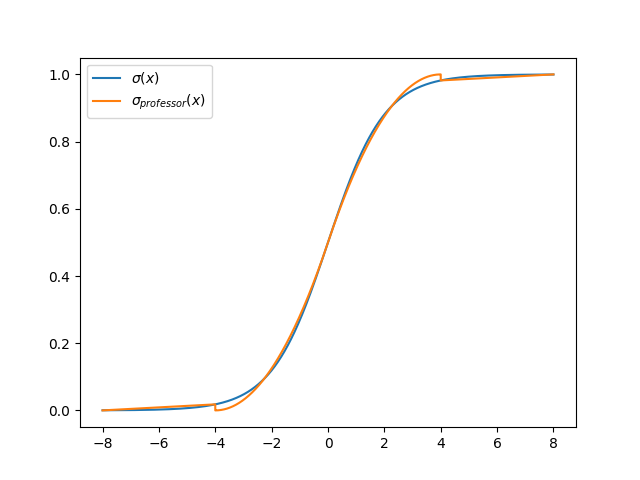
\includegraphics[scale=.7]{sig_prof.png}
\end{figure}
\end{center}

\section{Nova aproximação}

A segunda aproximação que realizei foi uma que eu mesmo criei. A ideia aqui é utilizar as propriedades simétricas da sigmoide disponíveis na equação \ref{eq:simetria}. Assim é necessário aproximar a sigmoide apenas para valores positivos, podendo extrapolar esta aproximação para valores negativos.

\begin{equation}
    \label{eq:simetria}
    \sigma(x) = 1 - \sigma(-x)
\end{equation}

Esta aproximação é feita dividindo o intervalo $[0, \infty]$ em três partes sendo duas lineares e uma não linear e, para isso é necessário ajustar dois parêmtros chamados aqui de $fim_l$ e $fim_n$. Assim, a equação \ref{eq:luis} define a função de aproximação.

\begin{equation}
    \label{eq:luis}
    \begin{split}
        y = 
        \begin{cases}
            1 + a_3  x - b_3, & x_{\inf} \leq x \leq -fim_n \\
            1 - c_2 + x  (-a_2  x + b_2), & -fim_n < x \leq -fim_l \\
            1 + a_1  x - b1, & -fim_l < x \leq 0 \\
            a_1  x + b_1, & 0 < valor \leq fim_l \\
            c_2 + x  (a_2  x + b_2), & fim_l < x \leq fim_n \\
            a_3  x + b_3, & fim_n < x \leq x_{\sup}
        \end{cases}
    \end{split}
\end{equation}

Desta forma, por mais que o valor de $y$ é dividido em 6 intervalos distintos, utilizamos a simetria para ser necessário parametrizar apenas 3 desses 6 intervalos. Os valalores $x_{\inf}$ e $x_{\sup}$, assim como na outra aproximação dependem das caracteristicas de ponto fixo utilizada, então não são parâmetros modificaveis, além disso nas definições das constantes utilizamos também o parâmetro $x_{med}$ que é a média entre $fim_l$ e $fim_n$. Os outros parâmetros podem ser calculados seguindo as fórmulas abaixo.

\begin{equation}
    \begin{split}
        a_1 =& \frac{\sigma(fim_l) - 0,5}{fim_l} \\
        b_1 =& \sigma(fim_l)
    \end{split}
\end{equation}

\begin{equation}
    \label{eq:coefs_n}
    \begin{split}
        a_2 = \dfrac{2 \sigma(fim_n) - 4 \sigma(x_{med}) + 2 \sigma(fim_n)}{(fim_n - fim_l)^2} \\
        b_2 = \frac{2 (\sigma(x_{med}) - \sigma(fim_l))}{fim_n - fim_l} - \frac{a_2}{2} \left( 3fim_l + fim_n\right) \\
        c_2 = \sigma(fim_n) - a_2 fim_l^2 - b_2 fim_l
    \end{split}
\end{equation}

\begin{equation}
    \begin{split}
        a_3 =& \frac{\sigma(fim_n) - x_{\sup}}{fim_n - x_{\sup}} \\
        b_3 =& \sigma(fim_n) - fim_n a_3
    \end{split}
\end{equation}

Dentro dos testes que realizei, os melhores resultados foram quando $fim_l = 0,7$ e $fim_n = 3,85$ obtendo assim um erro máximo de $0,87\%$ e um erro médio de $0,51\%$. A figura \ref{fig:meu} mostra a comparação de uma sigmoide real e desta aproximação.

\begin{center}
\begin{figure}[h]
\label{fig:meu}
    \caption{Comparação do segundo método com uma sigmoide real}
    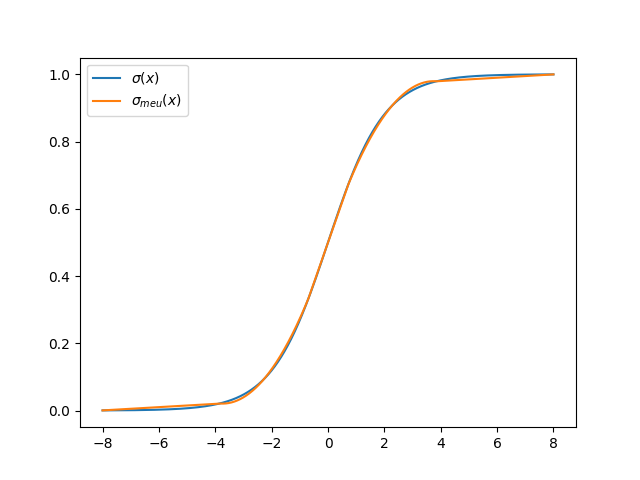
\includegraphics[scale=.7]{sig_meu.png}
\end{figure}
\end{center}

\subsection{Deduções}
Abordarei aqui como as deduções das constantes foram feitas para esta aproximação. Como pode ser visto na equação \ref{eq:luis} são criados 6 intervalos que, devido à simetria se tornam apenas 3. O primeiro intervalo linear ocorre com $x \in [0, fim_l]$, o segundo intervalo, esse não linear, ocorre com $x \in (fim_l, fim_n]$ e o último intervalo, linear, ocorre com $x \in (fim_n, x_{\sup}]$.

\subsubsection{Intervalos lineares}
Os intervalos lineares possuem uma dedução extremamente simples, apenas traçamos uma reta que passa pelos dois pontos que limitam o intervalo segundo a equação \ref{eq:reta}.

\begin{equation}
    \label{eq:reta}
   y - y_1= \frac{y_1 - y_2}{x_1 - x_2} (x - x_1)
\end{equation}

Realizaremos a dedução para a segunda parte linear, já que a da primeira é similar e inclusive mais simples. Substituindo na equação $y_1 = \sigma(fim_n)$, $y_2 = \sigma(x_{\sup})$, $x_1 = fim_n$ e $x_2 = x_{\sup}$ temos:

\begin{equation}
\begin{split}
    y - \sigma(fim_n) =& \frac{\sigma(fim_n) - \sigma(x_{\sup})}{fim_n - x_{\sup}}(x - fim_n) \\
    y =& \frac{\sigma(fim_n) - \sigma(x_{\sup})}{fim_n - x_{\sup}}(x - fim_n) + \sigma(fim_n) \\
    y =& \frac{\sigma(fim_n) - \sigma(x_{\sup})}{fim_n - x_{\sup}}x - fim_n \frac{\sigma(fim_n) - \sigma(x_{\sup})}{fim_n - x_{\sup}} + \sigma(fim_n) \\
\end{split}
\end{equation}

Considerando também a equação reduzida da reta: $y = ax + b$ podemos fazer as correspondências e obter que:

\begin{equation}
\begin{split}
    a =& \frac{\sigma(fim_n) - \sigma(x_{\sup})}{fim_n - x_{\sup}} \\
    b = - fim_n \frac{\sigma(fim_n) - \sigma(x_{\sup})}{fim_n - x_{\sup}} +& \sigma(fim_n) = \sigma(fim_n) - fim_n a
\end{split}
\end{equation}

\subsubsection{Intervalo não linear}
Neste intervalo tentamos definir a sigmoide como uma parábola e para tanto seria necessário três pontos, para isso escolhemos os limites do intervalo: $fim_l$, $fim_n$ e a média entre eles, assim definimos $x_1 = fim_l$, $x_2 = \dfrac{x_1 + x_2}{2}$ e $x_3 = fim_n$, além de que $y_1 = \sigma(x_1)$, $y_2 = \sigma(x_2)$ e $y_3 = \sigma(x_3)$. Desta forma foi possível escrever o sistema de equações abaixo:

\begin{equation}
\begin{split}
    y_1 =& ax_1^2 + bx_1 + c \\
    y_2 =& ax_2^2 + bx_2 + c \\
    y_3 =& ax_3^2 + bx_3 + c \\
\end{split}
\end{equation}

Esse sistema foi resolvido utilizando o método do escalonamento segundo as equações abaixo.

\begin{gather*}
\begin{bmatrix}
    1 & x_1 & x_1^2 & y_1 \\
    1 & x_2 & x_2^2 & y_2 \\
    1 & x_3 & x_3^2 & y_3 \\
\end{bmatrix}
\begin{matrix}
    \\
    L_2 = L_2 - L_1 \\
    L_3 = L_3 - L_1
\end{matrix} \\
\begin{bmatrix}
    1 & x_1       & x_1^2         & y_1 \\
    0 & x_2 - x_1 & x_2^2 - x_1^2 & y_2 - y_1\\
    0 & x_3 - x_1 & x_3^2 - x_1^2 & y_3 - y_1\\
\end{bmatrix}
\begin{matrix}
    \\
    \\
    L_3 = L_3 - \dfrac{x_3 - x_1}{x_2 - x_1}L_2
\end{matrix} \\
\begin{bmatrix}
    1 & x_1       & x_1^2         & y_1 \\
    0 & x_2 - x_1 & x_2^2 - x_1^2 & y_2 - y_1\\
    0 & 0         & x_3^2 - x_1^2 - \dfrac{(x_3 - x_1)}{(x_2 - x_1)}(x_2^2 - x_1^2) & y_3 - y_1 - \dfrac{(x_3 - x_1)}{(x_2 - x_1)}(y_2 - y_1)\\
\end{bmatrix} \\
\begin{bmatrix}
    1 & x_1       & x_1^2         & y_1 \\
    0 & x_2 - x_1 & x_2^2 - x_1^2 & y_2 - y_1\\
    0 & 0         & (x_3 - x_1)(x_3 + x_1) - \dfrac{(x_3 - x_1)\cancel{(x_2 - x_1)}(x_2 + x_1)}{\cancel{(x_2 - x_1)}} & y_3 - y_1 - \dfrac{(x_3 - x_1)}{(x_2 - x_1)}(y_2 - y_1)\\
\end{bmatrix} \\
\begin{bmatrix}
    1 & x_1       & x_1^2         & y_1 \\
    0 & x_2 - x_1 & x_2^2 - x_1^2 & y_2 - y_1\\
    0 & 0         & (x_3 - x_1) \left[\left(x_3 + x_1\right) - \left(x_2 + x_1\right)\right] & y_3 - y_1 - \dfrac{(x_3 - x_1)}{(x_2 - x_1)}(y_2 - y_1)\\
\end{bmatrix} \\
\begin{bmatrix}
    1 & x_1       & x_1^2         & y_1 \\
    0 & x_2 - x_1 & x_2^2 - x_1^2 & y_2 - y_1\\
    0 & 0         & (x_3 - x_1) (x_3 - x_2) & y_3 - y_1 - \dfrac{(x_3 - x_1)}{(x_2 - x_1)}(y_2 - y_1)\\
\end{bmatrix} \\
\end{gather*}

A partir daí foi possível encontrar os coeficientes $a$, $b$ e $c$ cujas expressões estão abaixo.

\begin{equation}
\begin{split}
    a = &\dfrac{y_3 - y_1}{(x_3 - x_1)(x_3 - x_2)} - \dfrac{y_2 - y_1}{(x_3 - x_2)(x_2 - x_1)} \\
    b = &\dfrac{y_2 - y_1}{x_2 - x_1} - a(x_2 + x_1) \\
    c = & y_1 - ax_1^2 - b x_1
\end{split}
\end{equation}

Por fim, novamente utilizando o fato de que $x_2 = \dfrac{x_1 + x_3}{2}$ simplificamos estas expressões para obter as expressões em \ref{eq:coefs_n}.
\end{document}
